\begin{center}

\includegraphics[width=0.5\textwidth]{content/3/chapter4/images/47.png}\\
Cippi goes up
\end{center}

This section presents the remaining small improvements in the C++20 core language.

\subsubsubsection{4.9.1\hspace{0.2cm} volatile}

The abstract in the proposal \href{http://www.open-std.org/jtc1/sc22/wg21/docs/papers/2018/p1152r0.html}{P1152R0} gives a short description of the changes that volatile undergoes: “The proposed deprecation preserves the useful parts of volatile, and removes the dubious / already broken ones. This paper aims at breaking at compile-time code which is today subtly broken at run time or through a compiler update.” Before I dive into volatile, I want to answer the crucial question: When should you use volatile?

A note from the C++ standard says that “volatile is a hint to the implementation to avoid aggressive optimization involving the object because the value of the object might be changed by means undetectable by an implementation.” This means that for a single thread of execution, the compiler must perform load or store operations in the executable as often as they occur in the source code. volatile operations, therefore, cannot be eliminated or reordered. Consequently, you can use volatile objects for communication with a signal handler but not for communication with another thread of execution.

Before I show you what semantics of volatile are preserved, I want to start with the deprecated features:

\begin{enumerate}
\item 
Deprecate volatile compound assignment, and pre/post increment/decrement

\item 
Deprecate volatile qualification of function parameters or return types

\item 
Deprecate volatile qualifiers in a structured binding declaration
\end{enumerate}

If you want to know all the sophisticated details, I strongly suggest you watch the CppCon 2019 talk \href{https://www.youtube.com/watch?v=KJW_DLaVXIY}{“Deprecating volatile”} from JF Bastien. Here are a few examples from his talk. Additionally, I fixed a few typos in the source code. The numbers in the following code snippets refer to the three deprecations listed earlier.

\hspace*{\fill} \\ %插入空行
\noindent
Deprecated use case for volatile
\begin{lstlisting}[style=styleCXX]
// (1)
int neck, tail;
volatile int brachiosaur;
brachiosaur = neck; // OK, a volatile store
tail = brachiosaur; // OK, a volatile load

// deprecated: does this access brachiosaur once or twice
tail = brachiosaur = neck;

// deprecated: does this access brachiosaur once or twice
brachiosaur += neck;

// OK, a volatile load, an addition, a volatile store
brachiosaur = brachiosaur + neck;

#########################################
// (2)
// deprecated: a volatile return type has no meaning
volatile struct amber jurassic();

// deprecated: volatile parameters aren't meaningful to the
// caller, volatile only applies within the function
void trex(volatile short left_arm, volatile short right_arm);

// OK, the pointer isn't volatile, the data it points to is
void fly(volatile struct pterosaur* pterandon);

########################################
(3)
struct linhenykus { volatile short forelimb; };
void park(linhenykus alvarezsauroid) {
	// deprecated: does the binding copy the forelimbs?
	auto [what_is_this] = alvarezsauroid; // structured binding
	// ...
}
\end{lstlisting}

\begin{tcolorbox}[colback=red!5!white,colframe=red!75!black,title={volatile and Multithreading Semantics}]
volatile is typically used to denote objects that can change independently of the regular program flow. These are, for example, objects in embedded programming that represent an external device (memory-mapped I/O). Because these objects can change independently of the regular program flow and their value is directly written to main memory, no optimized storing in caches takes place. In other words, volatile avoids aggressive optimization and has no multithreading semantics.
\end{tcolorbox}

\subsubsubsection{4.9.2\hspace{0.2cm} Range-based for loop with Initializers}

With C++20, you can directly use a range-based for loop with an initializer.

\hspace*{\fill} \\ %插入空行
\noindent
Range-based for loop with initializer
\begin{lstlisting}[style=styleCXX]
// rangeBasedForLoopInitializer.cpp

#include <iostream>
#include <string>
#include <vector>

int main() {

	for (auto vec = std::vector{1, 2, 3}; auto v : vec) {
		std::cout << v << " ";
	}
	
	std::cout << "\n\n";
	
	for (auto initList = {1, 2, 3}; auto e : initList) {
		e *= e;
		std::cout << e << " ";
	}
	
	std::cout << "\n\n";
	
	using namespace std::string_literals;
	for (auto str = "Hello World"s; auto c: str) {
		std::cout << c << " ";
	}
	
	std::cout << '\n';

}
\end{lstlisting}

The range-based for loop uses in line 9 a std::vector, in line 15 a std::initializer\_list, and in line 23 a std::string. Furthermore, in line 9 and line 15 I apply automatic type deduction for class templates, which we have since C++17. Instead of std::vector<int>, I just write std::vector.

\begin{tcblisting}{commandshell={}}
1 2 3

1 4 9

H e l l o  W o r l d
\end{tcblisting}

\begin{center}
Use of a range-based for loop
\end{center}

\subsubsubsection{4.9.3\hspace{0.2cm} Virtual constexpr function}

A constexpr function has the potential to run at compile time but can also be executed at run time. Consequently, you can make a constexpr function with C++20 virtual. Both directions are possible. A virtual constexpr function can override a non-constexpr function, and a virtual non-constexpr function can override a virtual constexpr function. I want to emphasize that override implies that the relevant function of a base class is virtual.

Program virtualConstexpr.cpp shows both combinations:

\hspace*{\fill} \\ %插入空行
\noindent
Virtual constexpr functions
\begin{lstlisting}[style=styleCXX]
// virtualConstexpr.cpp

#include <iostream>

struct X1 {
	virtual int f() const = 0;
};

struct X2: public X1 {
	constexpr int f() const override { return 2; }
};

struct X3: public X2 {
	int f() const override { return 3; }
};

struct X4: public X3 {
	constexpr int f() const override { return 4; }
};

int main() {
	
	X1* x1 = new X4;
	std::cout << "x1->f(): " << x1->f() << '\n';
	
	X4 x4;
	X1& x2 = x4;
	std::cout << "x2.f(): " << x2.f() << '\n';

}
\end{lstlisting}

Line 24 uses virtual dispatch (late binding) via a pointer, line 28 uses virtual dispatch via reference.

\begin{tcblisting}{commandshell={}}
x1->f(): 4
x2.f(): 4
\end{tcblisting}

\begin{center}
Use of virtual constexpr functions
\end{center}

\subsubsubsection{4.9.4\hspace{0.2cm} The new Character Type of UTF-8 Strings: char8\_t}

In addition to the character types char16\_t and char32\_t from C++11, C++20 gets the new character type char8\_t. Type char8\_t is large enough to represent any UTF-8 code unit (8 bits). It has the same size, signedness, and alignment as an unsigned char, but is a distinct type.

\begin{tcolorbox}[breakable,enhanced jigsaw,colback=blue!5!white,colframe=blue!75!black,title={char versus char8\_t}]
A char has one byte. In contrast to a char8\_t, the number of bits of a byte and hence of a char is not defined. Nearly all implementations use 8 bits for a byte. The std::string is an alias for a std::basic\_string of chars.

\hspace*{\fill} \\ %插入空行
\noindent
std::string and a std::string literal
\begin{lstlisting}[style=styleCXX]
std::string std::basic_string<char>
"Hello World"s
\end{lstlisting}
\end{tcolorbox}

Consequently, C++20 has a new typedef for the character type char8\_t (line 1) and a new UTF-8 string literal (line 2).

\hspace*{\fill} \\ %插入空行
\noindent
A new char8\_t character type and an UTF-8 string literal
\begin{lstlisting}[style=styleCXX]
std::u8string std::basic_string<char8_t>
u8"Hello World"
\end{lstlisting}

The program char8Str.cpp shows the straightforward usage of the new character type char8\_t.

\hspace*{\fill} \\ %插入空行
\noindent
Intuitive usage for the new character type char8\_t
\begin{lstlisting}[style=styleCXX]
// char8Str.cpp

#include <iostream>
#include <string>

int main() {
	
	const char8_t* char8Str = u8"Hello world";
	std::basic_string<char8_t> char8String = u8"helloWorld";
	std::u8string char8String2 = u8"helloWorld";
	
	char8String2 += u8".";
	
	std::cout << "char8String.size(): " << char8String.size() << '\n';
	std::cout << "char8String2.size(): " << char8String2.size() << '\n';
	
	char8String2.replace(0, 5, u8"Hello ");
	
	std::cout << "char8String2.size(): " << char8String2.size() << '\n';

}
\end{lstlisting}

Without further ado, here is the output of the program:

\begin{tcblisting}{commandshell={}}
char8String.size(): 10
char8String2.size(): 11
char8String2.size(): 12
\end{tcblisting}

\begin{center}
Use of the new character type char8\_t
\end{center}

\subsubsubsection{4.9.5\hspace{0.2cm} using enum in Local Scopes}

A using enum declaration introduces the enumerators of the named enumeration in the local scope.

\hspace*{\fill} \\ %插入空行
\noindent
Introducing enumerators in the local scope
\begin{lstlisting}[style=styleCXX]
// enumUsing.cpp

#include <iostream>
#include <string_view>

enum class Color {
	 red,
	 green,
	 blue
};

std::string_view toString(Color col) {
	switch (col) {
		using enum Color;
		case red: return "red";
		case green: return "green";
		case blue: return "blue";
	}
	return "unknown";
}

int main() {

	std::cout << '\n';
	
	std::cout << "toString(Color::red): " << toString(Color::red) << '\n';
	
	using enum Color;
	
	std::cout << "toString(green): " << toString(green) << '\n';
	
	std::cout << '\n';

}
\end{lstlisting}

The using enum declaration (line 14) introduces the enumerators of the scoped enumerations Color into the local scope. From that point on, the enumerators can be used unscoped (lines 15 - 17).

\begin{center}
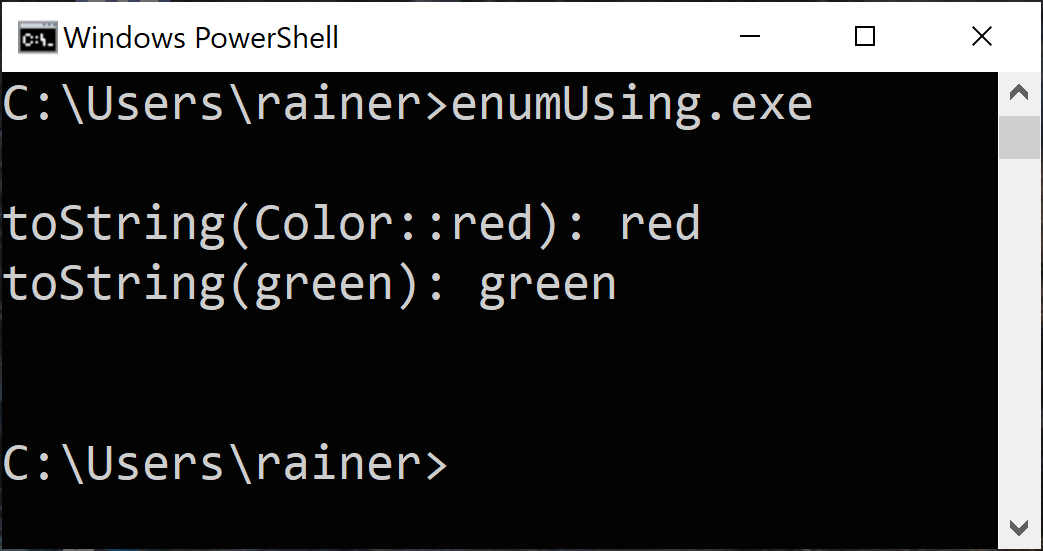
\includegraphics[width=0.8\textwidth]{content/3/chapter4/images/48.png}\\
Application of using enum
\end{center}

\subsubsubsection{4.9.6\hspace{0.2cm} Default Member Initializers for Bit Fields}

First of all, what is a bit field? Here is the definition from \href{https://en.wikipedia.org/wiki/Bit_field}{Wikipedia}: “A bit field is a data structure used in computer programming. It consists of a number of adjacent computer memory locations which have been allocated to hold a sequence of bits, stored so that any single bit or group of bits within the set can be addressed. A bit field is most commonly used to represent integral types of known, fixed bit-width.”

With C++20, we can default-initialize the members of a bit field:

\hspace*{\fill} \\ %插入空行
\noindent
Default initializers for the members of a bit field
\begin{lstlisting}[style=styleCXX]
// bitField.cpp

#include <iostream>

struct Class11 {
	int i = 1;
	int j = 2;
	int k = 3;
	int l = 4;
	int m = 5;
	int n = 6;
};

struct BitField20 {
	int i : 3 = 1;
	int j : 4 = 2;
	int k : 5 = 3;
	int l : 6 = 4;
	int m : 7 = 5;
	int n : 7 = 6;
};

int main () {
	
	std::cout << '\n';
	
	std::cout << "sizeof(Class11): " << sizeof(Class11) << '\n';
	std::cout << "sizeof(BitField20): " << sizeof(BitField20) << '\n';
	
	std::cout << '\n';

}
\end{lstlisting}

According to the members of a class (lines 6 - 11) with C++11, the members of bit field can have default initializers (lines 15 - 20) with C++20. When you sum up the numbers 3, 4, 5, 6, 7, and 7, you get 32. Hence, 32 bits, or 4 bytes is exactly the size of the BitField20:

\begin{center}
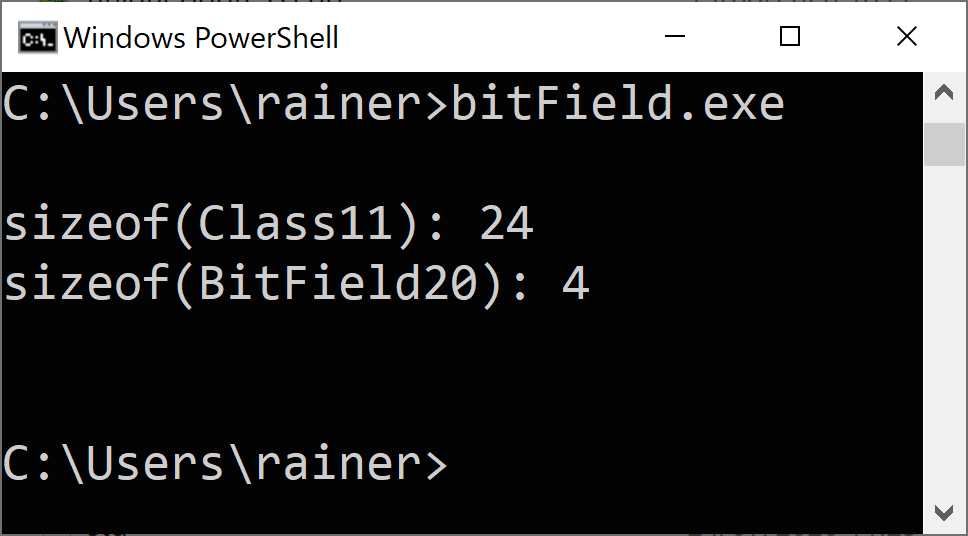
\includegraphics[width=0.6\textwidth]{content/3/chapter4/images/49.png}\\
Size information to a bit field
\end{center}

\begin{tcolorbox}[breakable,enhanced jigsaw,colback=mygreen!5!white,colframe=mygreen!75!black,title={Distilled Information}]
\begin{itemize}
\item 
The meaning of volatile is clarified in C++20. volatile has no multithreading semantics and should only be used to avoid aggressive optimization because an object may be changed independently of the regular program flow.

\item 
Range-based for loops can use an initializer.

\item 
The new character type char8\_t is large enough to represent 8 bits.

\item 
A using enum declaration introduces the enumerators of a named enumeration in the local scope.

\item 
The members of a bit field can be default-initialized.

\item 
A constexpr function can be virtual.
\end{itemize}
\end{tcolorbox}























